\documentclass[12pt]{article}
\usepackage{amssymb,amsmath}
\usepackage{times, verbatim}
\usepackage{graphicx}
\usepackage{epsfig}
\usepackage{epstopdf}
\usepackage{enumitem}
\usepackage{tabto}
\usepackage{xcolor}
\usepackage{hyperref}

\addtolength{\textwidth}{80pt}
\addtolength{\evensidemargin}{-40pt}
\addtolength{\oddsidemargin}{-40pt}
\addtolength{\topmargin}{-70pt}
\addtolength{\textheight}{1.75in}
\setlength{\parindent}{0in}
\setlength{\parskip}{10pt}
\hypersetup{
    colorlinks=true,
    linkcolor=blue,
    filecolor=magenta,      
    urlcolor=cyan,
}


\begin{document}
\normalsize
{\bf Joshua Chen}\\
{\bf GPS 5: Measles Model}\\
{\bf Mathematical Modelling}\\

{\bf Question 1:}\\
$S_{k+1} = S_k - \textcolor{red} {\alpha} I_k S_k + B = S_k(1 - \textcolor{red} {\alpha} I_k) + B $\\
$I_{k+1} = \textcolor{red} {\alpha} I_k S_k$\\

\textit{a) Complete the closed form:}\\
\normalsize $S_1 = S_0(1 - \textcolor{red} {\alpha} I_0) + B$\\\\
$S_2 = S_1(1 - \textcolor{red} {\alpha} I_1) + B = [S_0(1 - \textcolor{red} {\alpha} I_0) + B](1 - \textcolor{red} {\alpha} I_1) + B$\\
$\Rightarrow S_2 = S_0(1 - \textcolor{red} {\alpha} I_0)(1 - \textcolor{red} {\alpha} I_1) + (1 - \textcolor{red} {\alpha} I_1)B + B$\\\\
$S_3 = S_2(1 - \textcolor{red} {\alpha} I_2) + B =  [S_0(1 - \textcolor{red} {\alpha} I_0)(1 - \textcolor{red} {\alpha} I_1) + (1 - \textcolor{red} {\alpha} I_1)B + B](1 - \textcolor{red} {\alpha} I_2) + B$\\
$\Rightarrow S_3 = S_0(1 - \textcolor{red} {\alpha} I_0)(1 - \textcolor{red} {\alpha} I_1)(1 - \textcolor{red} {\alpha} I_2) + (1 - \textcolor{red} {\alpha} I_2)(1 - \textcolor{red} {\alpha} I_1)B +(1 - \textcolor{red} {\alpha} I_2)B + B$\\\\
$\Rightarrow S_3 = S_0 \displaystyle\sum^{2}_{i=0}(1 - \textcolor{red} {\alpha} I_i) + B(1 + (1 -\textcolor{red} {\alpha} I_2)(1 - \textcolor{red} {\alpha} I_1) + (1 - \textcolor{red} {\alpha} I_2))$\\
\hphantom{sjssfa} $= S_0\displaystyle\sum^{2}_{i=0}(1 - \textcolor{red} {\alpha} I_i) + B\left(1 + \displaystyle\sum^{2}_{j=1} \displaystyle \prod^{2}_{i=j}(1 - \textcolor{red} {\alpha} I_{i})\right)$\\
\begin{center}
Generalized Solution:
$S_k = S_0 \displaystyle\sum^{k-1}_{i=0}(1 - \textcolor{red} {\alpha} I_i) + B\left(1 + \displaystyle\sum^{k-1}_{j=1}\displaystyle \prod^{k-1}_{i=j}(1 - \textcolor{red} {\alpha} I_{i})\right)$\\
\end{center}
\begin{center}
\begin{tabular}{ c c c c c} 
blank 1:  $S_0$ & blank 2: $k-1$ & blank 3: $i = 0$ & blank 4: $\textcolor{red} {\alpha} I_i$  & blank 5 = B\\ 
blank 6: $k-1$ & blank 7: $j = 1$ & blank 8: $k - 1$ & blank 9: $i = j$ &blank 10: $\textcolor{red} {\alpha} I_{i}$ \\\\
\end{tabular}
\end{center}

\textit{b) Find the fixed points:}\\
Let $S^* = S_k = S_{k+1}$\\
Let $I^* = I_k = I_{k+1}$\\\\
$S^* = S^*(1 - \textcolor{red} {\alpha} I^*) + B$\\
$I^* = \textcolor{red} {\alpha} I^* S^*$\\
From the second equation, we can derive that $S^* = \cfrac{1}{\textcolor{red} {\alpha}}$\\
If we multiply the first equation by $\textcolor{red} {\alpha}$, we get $1 = (1 - \textcolor{red} {\alpha} I^*) + B\textcolor{red} {\alpha}$\\
$\textcolor{red} {\alpha} I^* =B\textcolor{red} {\alpha}$\\
$I^* = B$
\begin{center}
\begin{tabular}{ c c c } 
& At the fixed points: &\\
$S^* = \cfrac{1}{\textcolor{red} {\alpha}}$ & & $I^* = B$\\
\end{tabular}
\end{center}
\break
\textit{c) Apply the Jacobian to check stability by testing eigenvalues at fixed points.}
\begin{center}
$\textcolor{red} {\alpha} = 0.00003 \qquad B = 120$\\
\end{center}
$f(S_k,I_k) = S_k - \textcolor{red} {\alpha} I_k S_k + B \quad \Rightarrow \quad$
\begin{tabular}{c c c}
$\cfrac{\partial f}{\partial S_k} = 1 - \textcolor{red} {\alpha} I_k$ &  $\quad \cfrac{\partial f}{\partial I_k} = -\textcolor{red} {\alpha} S_k$\\
\end{tabular}
\\\\\\\
$g(S_k,I_k) = \textcolor{red} {\alpha} I_k S_k \quad \qquad \Rightarrow \qquad$
\begin{tabular}{c c}
$\quad \cfrac{\partial g}{\partial S_k} = \textcolor{red} {\alpha} I_k$ & $\quad \cfrac{\partial g}{\partial I_k} = \textcolor{red} {\alpha} S_k$\\
\end{tabular}
\begin{center}
$J
\begin{pmatrix}
f(S_k,I_k)\\
g(S_k,I_k)\\
\end{pmatrix}
= \begin{pmatrix}
1-\textcolor{red} {\alpha} I_k & -\textcolor{red} {\alpha} S_k\\
\textcolor{red} {\alpha} I_k & \textcolor{red} {\alpha} S_k\\
\end{pmatrix}$
\end{center}

At the fixed point $\left(S^* = \cfrac{1}{\textcolor{red} {\alpha}}, I^* = B\right)$:
$\qquad J
\begin{pmatrix}
f(S_k,I_k)\\
g(S_k,I_k)\\
\end{pmatrix}
= \begin{pmatrix}
1- \textcolor{red} {\alpha} B & -1\\
\textcolor{red} {\alpha} B & 1\\
\end{pmatrix}$

After plugging in $\textcolor{red} {\alpha}$ and $B$:
$\qquad J
\begin{pmatrix}
f(S_k,I_k)\\
g(S_k,I_k)\\
\end{pmatrix}
= \begin{pmatrix}
0.9964 & -1\\
0.0036 & 1\\
\end{pmatrix}$\\\\
Using a \href{https://www.symbolab.com/solver/matrix-eigenvalues-calculator}{matrix calculator}, we can find eigenvalues satisfy the equation: $\lambda^2-1.9964\lambda+1 = 0$ \\
\hphantom{sjssfa} $\lambda = 0.9982+0.05997\dots i,\: \lambda=0.9982-0.05997\dots i$\\
Modulus $= \sqrt{(0.9982-0.05997i)(0.9982+0.05997i)} = 0.79797$
\begin{center}
$0.79797 < 1$ so the model is stable at the fixed points.
\end{center}

\break
\textit{d) Graph results}:
\begin{center}
\normalsize $S_0 = 30,000 \quad I_0 = 20 \quad \textcolor{red} {\alpha} = 0.00003 \quad B = 120$
\end{center}
\begin{center}
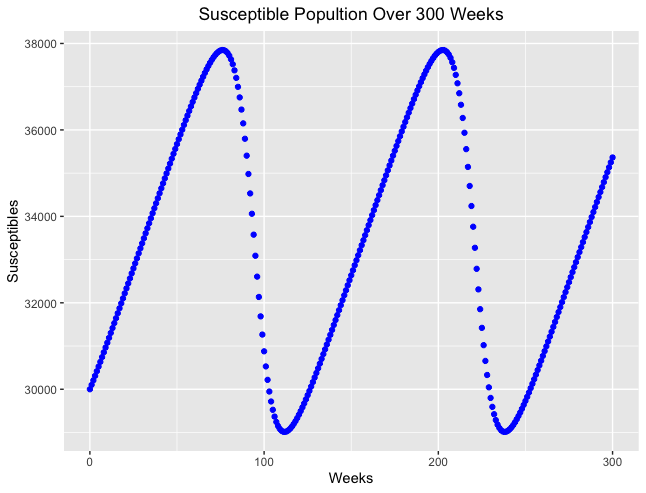
\includegraphics[width=12cm, ]{susceptible.png}
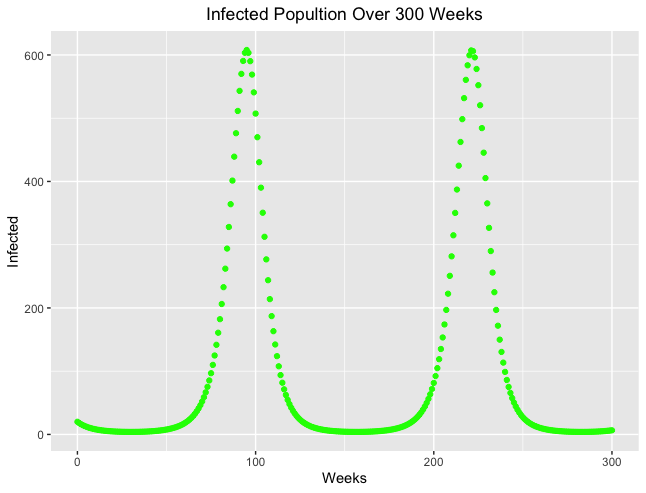
\includegraphics[width=12cm, ]{infected.png}
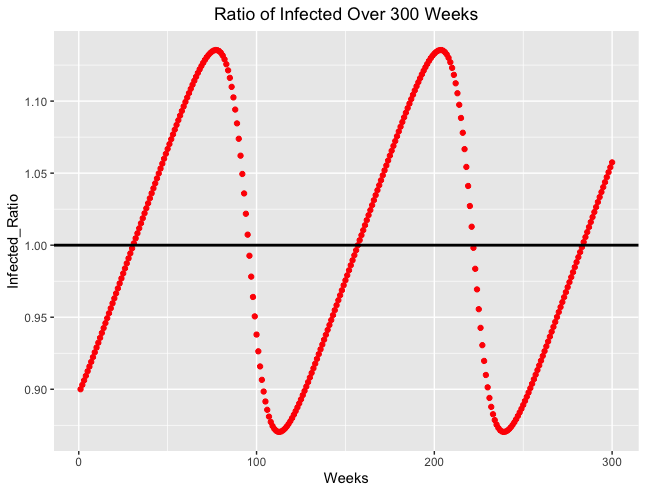
\includegraphics[width=12cm, ]{ratio_infected.png}
\end{center}

$\cfrac{I_{k+1}}{I_k}$ falls just below 1 at weeks 96 and 222. At these points, the number of infected people starts to decrease and the population of susceptible people starts to accelerate.\\\\
At the peaks, the number of infected is around 608 people. The number of susceptible people at this point is just under 32800 and the ratio $\cfrac{I_{k+1}}{I_k} \approx 1$\\\\
A constant birth rate of 120 people stops the number of susceptible people from ever reaching zero.\\\\\\\\\
\begin{center}
\small \href{https://github.com/chenjoshua7/SIR_model_measles/blob/master/Problem%201/Datasets/GPS5_master_data.csv}{The dataset used to construct the graphs can be accessed through this link.}
\end{center}
\break
{\bf Question 2:}\\
$S_{k+1} = S_k - \textcolor{red} {\alpha} I_k S_k + B_k = S_k(1 - \textcolor{red} {\alpha} I_k) + B_k $\\
$I_{k+1} = \textcolor{red} {\alpha} I_k S_k$\\
$B_{k+1} = \textcolor{red}{c} B_k$\\

\textit{a) Complete the closed form:}\\\\
\normalsize $S_1 = S_0(1 - \textcolor{red} {\alpha} I_0) + B_0$\\\\
$S_2 = S_1(1 - \textcolor{red} {\alpha} I_1) + B_1 = [S_0(1 - \textcolor{red} {\alpha} I_0) + B_0](1 - \textcolor{red} {\alpha} I_1) + B_1$\\
$\Rightarrow S_2 = S_0(1 - \textcolor{red} {\alpha} I_0)(1 - \textcolor{red} {\alpha} I_1) + (1 - \textcolor{red} {\alpha} I_1)B_0 + B_1$\\\\
$S_3 = S_2(1 - \textcolor{red} {\alpha} I_2) + B_2 =  [S_0(1 - \textcolor{red} {\alpha} I_0)(1 - \textcolor{red} {\alpha} I_1) + (1 - \textcolor{red} {\alpha} I_1)B_0 + B_1](1 - \textcolor{red} {\alpha} I_2) + B_2$\\
$\Rightarrow S_3 = S_0(1 - \textcolor{red} {\alpha} I_0)(1 - \textcolor{red} {\alpha} I_1)(1 - \textcolor{red} {\alpha} I_2) + (1 - \textcolor{red} {\alpha} I_2)(1 - \textcolor{red} {\alpha} I_1)B_0 +(1 - \textcolor{red} {\alpha} I_2)B_1 + B_2$\\\\
$\Rightarrow S_3 = S_0 \displaystyle\sum^{2}_{i=0}(1 - \textcolor{red} {\alpha} I_i) + B_2 + (1 - \textcolor{red} {\alpha} I_2)B_1 + (1 -\textcolor{red} {\alpha} I_2)(1 - \textcolor{red} {\alpha} I_1)B_0$\\
\hphantom{sjssfa} $= S_0\displaystyle\sum^{2}_{i=0}(1 - \textcolor{red} {\alpha} I_i) + \left( \displaystyle\sum^{2}_{j=0} B_j \displaystyle \prod^{2}_{i=j+1}(1 - \textcolor{red} {\alpha} I_{i})\right)$\\
\begin{center}
Generalized Solution:
$S_k = S_0 \displaystyle\sum^{k-1}_{i=0}(1 - \textcolor{red} {\alpha} I_i) + \left(\displaystyle\sum^{k-1}_{j=0}B_{j}\displaystyle \prod^{k-1}_{i=j+1}(1 - \textcolor{red} {\alpha} I_{i})\right)$\\
\end{center}
\begin{center}
\begin{tabular}{ c c c c c} 
blank 1:  $S_0$ & blank 2: $k-1$ & blank 3: $i = 0$ & blank 4: $\textcolor{red} {\alpha} I_i$  & blank 5 = k-1\\ 
blank 6: $j=0$ & blank 7: $B_{j}$ & blank 8: $k - 1$ & blank 9: $i = j + 1$ &blank 10: $\textcolor{red} {\alpha} I_{i}$ \\\\
\end{tabular}
\end{center}



\break
\textit{b) Graph produced:}
\begin{center}
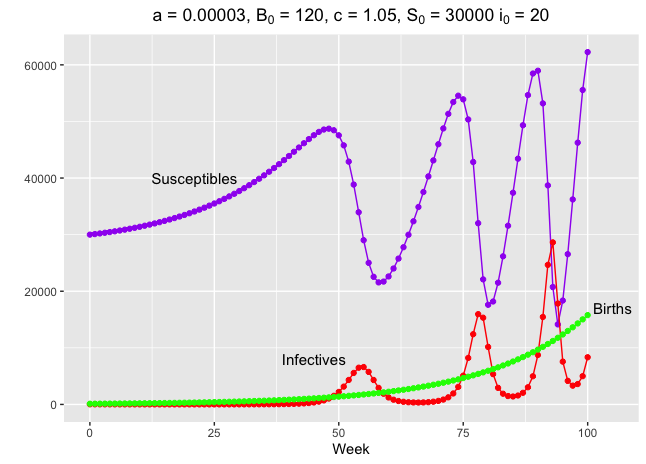
\includegraphics[width=15cm, ]{question2.png}
\end{center}

\begin{center}
At each peak: $\quad$
\begin{tabular}{ c | c c c c }
Week & $48$  & $74$ & $90$ & $101$\\
\hline
Susceptible & $48570.28$ & $53428.76$ & $58469.86$ & $62254.86$\\
\end{tabular}
\end{center}
The first finite difference is roughly equivalent to the first derivative. Therefore, when the sign becomes negative at these points, the number of infectives begins to decrease.\\


\textit{c) Explain the graph's behavior in the last 7 weeks:}\\
Because of $S_k$ and $I_k$ are all dependent on $B_k$ and $B_k$ is an exponentially growing function, toards the end of the graph, $I_k$ and $S_k$ oscillate more and more towards the end, due to more and more births. Eventually, when the birth rate is high enough, the population of susceptible and infective will begin to intersect, as we see in the last 7 weeks.

\begin{center}
\small \href{https://github.com/chenjoshua7/SIR_model_measles/blob/master/Problem%202/GPS5_Problem2_data.csv}{The dataset used to construct the graphs can be accessed through this link.}\\
\end{center}

\begin{center}
\normalsize All datasets and graphs were constructed in R through RStudio, These files, as well as the LaTeX files, can be found \href{https://github.com/chenjoshua7/SIR_model_measles}{here}.
\end{center}



\end{document}
